\documentclass[10pt,a4paper]{article}
%\documentclass[10pt,letter]{article}
\usepackage[left=1.5cm,top=1.5cm,right=1.5cm,bottom=1.5cm,nohead]{geometry}
%\usepackage{hyperref}
%\usepackage{helvet}
%\renewcommand{\familydefault}{\sfdefault}
\usepackage{graphicx}
\usepackage[parfill]{parskip}
\linespread{1.3}
\usepackage{amsmath}
\usepackage[authoryear,round]{natbib}
\renewcommand{\arraystretch}{1.3} % Extra spacing in arrays
\usepackage{lineno}  % Add this package

\linenumbers  % This turns line numbering on

\begin{document}
\begin{center}
	
\begin{figure}[t]
    \begin{center}
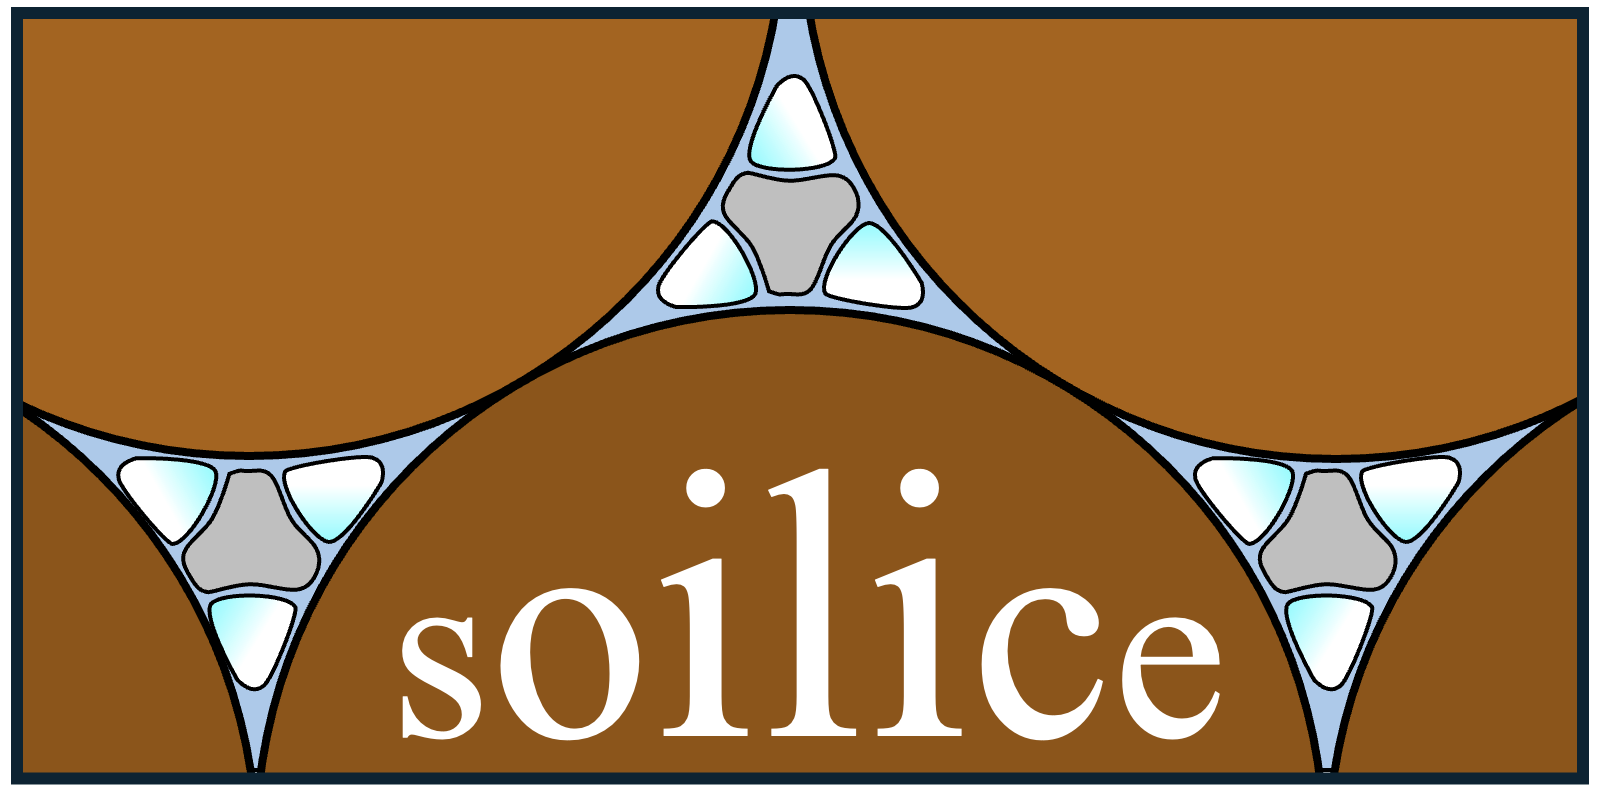
\includegraphics[width=8.3cm]{../logo.png}
    \end{center}
\end{figure}


{\huge soilice: Governing Equations}\\
\vspace{12pt}
{\large Andrew Ireson}\\
%{\large Alana Muenchrath}\\
%{\large Chris Spence}\\
%{\large Simon Mathias}\\
\vspace{12pt}
\today

\end{center}

\section{State variables}

We assume the following soil volume, mass, energy and temperature relations, all of which are extensive variables:

\begin{equation}
	\begin{array}{l}
		V=V_I+V_L+V_S+V_A \\
		M=M_I+M_L+M_S+M_A\\
		U=U_I+U_L+U_S+U_A\\
		T=T_I=T_L=T_S=T_A
	\end{array}
\end{equation}

where $V$ (m$^3$) is volume, $M$ (kg) is mass, $U$ (J) is internal energy and $T$ ($^\circ$C) is temperature, and subscripts are for the components liquid, $L$, ice, $I$, soil solid matter, $S$, and air, $A$. 

Equivalent intensive variables, expressed per unit volume, and given by dividing the above expressions (excluding $T$) by $V$ are

\begin{equation}
	\begin{array}{l}
		V/V=1=\theta_I+\theta_L+\theta_S+\theta_A \\
		M/V=m=m_I+m_L+m_S+m_A\\
		U/V=u=u_I+u_L+u_S+u_A\\
	\end{array}
\end{equation}


The density of a component, $\rho_i$ (kg m$^{-3}$), is

\begin{equation}
	\rho_i=\frac{M_i}{V_i}
\end{equation}

while the mass fraction of a component, $m_i$ (kg m$^{-3}$) is

\begin{equation}
	m_i=\frac{M_i}{V}=\rho_i\theta_i
\end{equation}

\section{Internal energy}

Consider a control volume of water $V$ (m$^3$), of mass $M$ (kg) and temperature $T$ ($^\circ$C). We define internal energy associated with sensible heat, that is the sensible internal energy, $U_s$ (J), as 

\begin{equation}
U_s=M c_pT
\end{equation}

where $c_p$ (J kg$^{-1}$ K$^{-1}$) is the specific heat capacity (which is defined by this equation). Likewise


\begin{equation} \label{eq: SH}
u_s=m c_pT
\end{equation}

The differential equation for the change in sensible internal energy with time is

\begin{equation}
\frac{du_s}{dt}=\frac{d}{dt}(m c_p T)=m c_p \frac{dT}{dt} + c_p T \frac{dm}{dt}
\end{equation}

Latent heat is a form of internal energy, called latent internal energy, $U_l$ (J), associated with the chemical bonds between molecules in a particular phase (solid, liquid, gas) of a substance. We assume latent heat is negative in the solid phase, zero in the liquid phase and positive in the vapor phase, hence

\begin{equation}
	\begin{array}{c}
	U_{li}=-M_i\lambda_f
	\\
	U_{ll}=0
	\\
	U_{lv}=M_v\lambda_v
	\end{array}
\end{equation}

where $\lambda_f$, the amount of heat needed to convert 1 kg of ice to 1 kg of liquid water, is a constant $\approx 3.34\times10^5$ J kg$^{-1}$ and $\lambda_v=2.50\times10^6$ J kg$^{-1}$ at $T=0^\circ$C). Likewise, we can define the intensive variables:

\begin{equation}
	\begin{array}{c}
	u_{li}=-u_i\lambda_f
	\\
	u_{ll}=0
	\\
	u_{lv}=m_v\lambda_v
	\end{array}
\end{equation}

Using this convention, the total latent internal energy is

\begin{equation} \label{eq: u_l_rel}
u_l=-m_i \lambda_f +m_v \lambda_v
\end{equation}

and the change in latent internal energy is

\begin{equation}
\frac{du_l}{dt}=-\lambda_f\frac{dm_i}{dt}+\lambda_v\frac{dm_v}{dt}
\end{equation}

The total internal energy that concerns us in soils is given by the sum of sensible and latent heat, i.e.

\begin{equation}
u=u_s+u_l
\end{equation}

In a control volume containing ice, liquid water, vapor and soil solids we have 

\begin{equation}
u=u_{si}+u_{sl}+u_{sv}+u_{ss}+u_{li}+u_{lv}
\end{equation}

(Noting that $U_{ll}=0$). 

\section{Mass and energy balance equations}

We will assume that the mass and internal energy in the vapor phase is negligible, hence

\begin{equation}
\begin{array}{l}
	m_v=0\\
	u_{sv} = 0\\
	u_{lv} = 0
\end{array}
\end{equation}

The mass and energy balance equations are 

\begin{equation} \label{eq: FD_massbal}
\frac{dm}{dt}=\frac{dm_l}{dt}+\frac{dm_i}{dt}=-\nabla q_l\rho_l
\end{equation}

and 

\begin{equation}
\frac{du}{dt}=
\frac{du_{si}}{dt}+
\frac{du_{sl}}{dt}+
\frac{du_{ss}}{dt}+
\frac{du_{li}}{dt}=
-\nabla (j_a+j_c+j_o)
\end{equation}

where $q_l$ (m s$^{-1}$) is the flux of liquid water and $j_a$, $j_c$ and $j_o$ (J m$^{-2}$ s$^{-1}$) are the advective, conductive, and other heat flux components. Expanding the left hand side of the energy balance equation gives

\begin{equation} \label{eq: UBal3DP}
	\begin{array}{ll}
		\displaystyle
\frac{du}{dt}
&
		\displaystyle
=\left(m_{i} c_{pi} + m_{l} c_{pl} + m_{s} c_{ps}\right)
\frac{dT}{dt}
+c_{pl}T
\frac{dm_{l}}{dt}
+(c_{pi}T-\lambda_f)
\frac{dm_i}{dt}\\
	\end{array}
\end{equation}

We define the bulk heat capacity, $c_{pb}$ (J kg$^{-1}$ K$^{-1}$) as

\begin{equation}
c_{pb}=m_{i} c_{pi} + m_{l} c_{pl} + m_{s} c_{ps}
\end{equation}

so we have 

\begin{equation} \label{eq: UBal3DP}
	\begin{array}{ll}
		\displaystyle
\frac{du}{dt}
&
		\displaystyle
=c_{pb}
\frac{dT}{dt}
+c_{pl}T
\frac{dm_{l}}{dt}
+(c_{pi}T-\lambda_f)
\frac{dm_i}{dt}\\
	\end{array}
\end{equation}


Now we want to eliminate the terms $dm_l/dt$ and $dm_i/dt$. Under equilibrium conditions (which is a big assumption) a soil control volume should reach a unique state on the basis of the temperature and the total water. We ignore any hysteresis effects. We define the total water content, $\theta_T$ (-) as being given by

\begin{equation}
	\theta_T=\theta_L+\frac{\rho_I}{\rho_L}\theta_I
\end{equation}

We defined $\psi_e$ (m) as the effective matric potential, which is associated with $\theta_T$ by the soil characteristic curve relationship, 

\begin{equation}
	\theta_T=\theta(\psi_e)
\end{equation}

$\psi_f$ (m) is the matric potential that corresponds to the freezing threshold, as defined by the GCE, where (Amankwah et al., 2021):

\begin{equation}
	\psi_f=\frac{\lambda_f}{g}\ln\left(\frac{T+T_0}{T_0}\right)
\end{equation}

where $T$ is the soil temperature in $^\circ$C, and $T_0 = 273.15$. If $\psi_e\leq\psi_f$ there is no ice in the soil pore space. Now we say 

\begin{equation}
	\begin{array}{llll}
		\theta_T=\theta(\psi_e); & \theta_L=\theta_T; & \theta_I = 0; & \mathrm{if}\hspace{6pt} \psi_e\leq\psi_f\\
		\\
		\theta_T=\theta(\psi_e); & \theta_L=\theta(\psi_f(T))=F(T); & \theta_I = \frac{\rho_L}{\rho_I}(\theta_T-\theta_L); & \mathrm{if}\hspace{6pt} \psi_e>\psi_f\\
	\end{array}
\end{equation}

The function $F(T)$ defines the freezing characteristic curve, and is simply the combination of the GCE and the $\theta(\psi)$ relationship. $\theta(\psi)$ and $F(T)$ can be differentiated, giving

\begin{equation}
	\frac{d\theta_T}{d\psi_e}=C(\psi_e)
\end{equation}

and

\begin{equation}
	\frac{d\theta_{L}}{dT}=F'(T)
\end{equation}

So we can further say

\begin{equation} \label{eq_thetaPart}
	\begin{array}{llll}
		\displaystyle \frac{d\theta_T}{dt} = C(\psi_e)\frac{d\psi_e}{dt};
		& \displaystyle \frac{d\theta_L}{dt} = \frac{d\theta_T}{dt};
		& \displaystyle \frac{d\theta_I}{dt} = 0;
		& \displaystyle \mathrm{if}\hspace{6pt} \psi_e\leq\psi_f\\
		\\
		\displaystyle \frac{d\theta_T}{dt} = C(\psi_e)\frac{d\psi_e}{dt};
		& \displaystyle \frac{d\theta_L}{dt} = F'(T)\frac{dT}{dt};
		& \displaystyle \frac{d\theta_I}{dt} = \frac{\rho_L}{\rho_I}\left(\frac{d\theta_T}{dt}-\frac{d\theta_L}{dt}\right);
		& \displaystyle \mathrm{if}\hspace{6pt} \psi_e>\psi_f\\
	\end{array}
\end{equation}

Now, consider first the case where $\psi_e \leq \psi_f$ (i.e. the soil is unfrozen). We have 

\begin{equation}
	\begin{array}{cc}
\displaystyle \frac{dm_l}{dt}=\frac{dm}{dt};
& 
\displaystyle \frac{dm_i}{dt}=0
	\end{array}
\end{equation}
%
Substituting this into Equation \ref{eq: UBal3DP} we have

\begin{equation} \label{eq: unfrozen_dT}
\frac{dT}{dt}
=
\frac{\displaystyle\frac{du}{dt}
-c_{pl}T
\frac{dm}{dt}
}{c_{pb}
}
\end{equation}

Next consider the case where $\psi_e > \psi_f$ (i.e. the soil is frozen). This time we have

\begin{equation}
\frac{dm_l}{dt}=\rho_lF'(T)\frac{dT}{dt}
\end{equation}

and

\begin{equation}
\frac{dm_i}{dt}=\frac{dm}{dt}-\frac{dm_l}{dt}
=
\frac{dm}{dt}-\rho_lF'(m,T)\frac{dT}{dt}
\end{equation}

Substituting these expressions into the Equation \ref{eq: UBal3DP} we get

%\begin{equation} 
%\frac{du}{dt}
%=
%(c_{pb}
%+\rho_l F'(T)
%((c_{pl}-c_{pi})T+\lambda_f)
%)\frac{dT}{dt}
%+(c_{pi}T-\lambda_f)
%\frac{dm}{dt}
%\end{equation}
%
%Rearranging we have

\begin{equation} \label{eq: frozen_dT}
\frac{dT}{dt}
=
\frac{\displaystyle
\frac{du}{dt}
-(c_{pi}T-\lambda_f)
\frac{dm}{dt}
}{c_{pb}
+\rho_l F'(T)
((c_{pl}-c_{pi})T+\lambda_f)
}
\end{equation}

which may then be solved by replacing the derivative terms on the right hand side with the net fluxes.

\section{Finite difference formulation}

For a one-dimensional vertical model, with $z$ (m) representing the depth below the ground surface, it is good practice to use a block-centred grid, where $z_n$ denotes the midpoint of a cell, and $z_{n-1/2}$ and $z_{n+1/2}$ are the depths of the top and bottom faces of the cell, respectively. Considering a single control volume at depth index $n$, we can write

\begin{equation} \label{eq: massAndEnergy}
	\begin{array}{rcl}
		\displaystyle
\left . \frac{dm_l}{dt}\right |_n
+ \left . \frac{dm_i}{dt}\right |_n
& 
\displaystyle 
= -\rho_l\nabla q_n
%&
%		\displaystyle
%=\frac{(q_{l,n-1/2}-q_{l,n+1/2})\rho_l}{z_{n+1/2}-z_{n-1/2}}
\\[1.0em]
		\displaystyle
\left . \frac{du}{dt}\right |_n
& 
\displaystyle 
= -\nabla j_n
%&
%		\displaystyle
%=\frac{(j_{a,n-1/2}-j_{a,n+1/2})
%+(j_{c,n-1/2}-j_{c,n+1/2})
%+(j_{o,n-1/2}-j_{o,n+1/2})
%}{z_{n+1/2}-z_{n-1/2}}
	\end{array}
\end{equation}

where $\nabla q_n$ and $\nabla j_n$ are the net fluxes of mass and energy into the control volume. Expressing these equations with total mass, $m$ and temperature $T$ as the dependent variables we have 

\begin{equation} 
\left . \frac{dm}{dt} \right |_n
=-\rho_l \nabla q_n
\end{equation}

\begin{equation} 
\left . \frac{dT}{dt} \right |_n
=
\left \{
	\begin{array}{ll}
\displaystyle
\frac{ \nabla j_n
-c_{pl}T_n
\left . \frac{dm}{dt} \right |_n
}{c_{pb}
}
,
&\displaystyle  \psi_{e,n} \leq \psi_{f,n}
\\[1.0em]
\displaystyle
\frac{\nabla j_n
-(c_{pi}T_n-\lambda_f)
\left . \frac{dm}{dt} \right |_n
}{c_{pb}
+\rho_l f'(m_n,T_n)
((c_{pl}-c_{pi})T_n+\lambda_f)
}
,
&\displaystyle \psi_{e,n} > \psi_{f,n}
	\end{array}
\right .
\end{equation}

Expanding the flux terms we have

\begin{equation} \label{eq: massAndEnergy}
	\begin{array}{rl}
\displaystyle 
-\rho_l\nabla q_n
&
		\displaystyle
=\frac{(q_{l,n-1/2}-q_{l,n+1/2})\rho_l}{z_{n+1/2}-z_{n-1/2}}
\\[1.0em]
\displaystyle 
-\nabla j_n
&
		\displaystyle
=\frac{(j_{a,n-1/2}-j_{a,n+1/2})
+(j_{c,n-1/2}-j_{c,n+1/2})
+(j_{o,n-1/2}-j_{o,n+1/2})
}{z_{n+1/2}-z_{n-1/2}}
	\end{array}
\end{equation}

Here the individual flux terms are given by

\begin{equation}
\begin{array}{rl}
	\displaystyle
q_{l,n-1/2}&\displaystyle =-K_{n-1/2}\left(\frac{\psi_n-\psi_{n-1}}{z_i-z_{n-1}}-1\right)
\\[0.8em]
	\displaystyle
q_{l,n+1/2}&\displaystyle =-K_{n+1/2}\left(\frac{\psi_{n+1}-\psi_{n}}{z_{n+1}-z_{n}}-1\right)
\\[0.8em]
	\displaystyle
j_{a,n-1/2}&\displaystyle =q_{l,n-1/2}\rho_l c_{pl} T_{n-1}
\\[0.8em]
	\displaystyle
j_{a,n+1/2}&\displaystyle =q_{l,n+1/2}\rho_l c_{pl} T_{n}
\\[0.8em]
	\displaystyle
j_{c,n-1/2}&\displaystyle =-\kappa_{n-1/2}\left(\frac{T_n-T_{n-1}}{z_n-z_{n-1}}\right)
\\[0.8em]
	\displaystyle
j_{c,n+1/2}&\displaystyle =-\kappa_{n+1/2}\left(\frac{T_{n+1}-T_{n}}{z_{n+1}-z_{n}}\right)
\end{array}
\end{equation}

For the advected heat fluxes here we assume the water flux is positive in the $z$ direction, such that $T_{n-1}$ is the downstream temperature at point $n-1/2$, and $T_n$ is the upstream temperature at point $n+1/2$. Alternative formulations for advection may be considered, but we will not expand on this here.  The term $j_o$ will be zero for all $n$ except $n=1$, that is the upper boundary condition (i.e. $j_{o,1/2}\neq 0$). 

Consider a soil profile subject to a vertical infiltration flux $q_a$ (m s$^{-1}$), a drainage flux, $q_d$ (m s$^{-1}$) and an evaporative loss term $q_e$ (m s$^{-1}$). The following boundary conditions can be used, where index $n=1$ represents the ground surface and $n=N$ is the lower boundary: 

\begin{equation} \label{eq: BCs}
	\begin{array}{rl}
q_{l,1/2}& =q_a-q_e
\\
q_{l,N+1/2}& =q_d
\\
j_{a,1/2}& =j_{a,T}
\\
j_{c,1/2}& =j_{g,T}
\\
j_{a,N+1/2}& =j_{a,B}
\\
j_{c,N+1/2}& =j_{g,B}
\\
j_{o,1/2}& =j_r-j_h-j_e
\\
j_{o,N+1/2}& =0
	\end{array}
\end{equation}

where all $j$ terms have units (J m$^{-2}$ s$^{-1}$), and $j_{a,T}$ is advection with net infiltrating water, $j_{g,T}$ is the ground heat flux, driven by conduction across the soil surface (important when there is snow on the ground), $j_r$ is net radiation, $j_h$ is the sensible heat lost (advection with the movement of air), $j_e$ is the latent heat lost to evaporation (advection of water vapor),  $j_{a,B}$ is advection with water draining out the base of the soil and $j_{g,B}$ is the conductive heat flux across the lower boundary. The different flux terms in Eq \ref{eq: BCs} may be zero under different scenarios (e.g. snow cover, bare soil, etc) or assumptions. 

We have here a system of ordinary differential equations which we solve using an ODE solver with the method of lines. 

\section{Hydraulic and thermal properties}

Now, we need expressions for $M$, $M'$, $F$ and $F'$, all of which we can get from the van Genuchten equations combined with the GCE equation.

\begin{equation}
S_e=(1+(\alpha \psi)^n)^{-m}\end{equation}

\begin{equation}
\theta=M(\psi)=\theta_r+(\theta_{sat}-\theta_r)S_e\end{equation}

\begin{equation}
\frac{d\theta}{d\psi}=M'(\psi)=
\frac{-\alpha m (\theta_{sat}-\theta_r)}{1-m}
S_e^{1/m}\left(1-S_e^{1/m}\right)^m
\end{equation}

The GCE:

\begin{equation}
\psi_f(T)=\frac{\lambda_f}{g}\ln\left(\frac{T+T_0}{T_0}\right)\approx\frac{L_f}{g}\left(\frac{T}{T_0}\right)\end{equation}

and 

\begin{equation}
\begin{array}{ll}
	F(T) & =M\left(\psi_f(T)\right)
	% = \theta_r+(\theta_{sat}-\theta_r)\left(1+(\alpha\psi_f)^n\right)^{-m}
	\\
	& =
	\theta_r+(\theta_{sat}-\theta_r)\left(1+\left(
	\frac{\alpha L_fT}{gT_0}
	\right)^n\right)^{-m}
\end{array}
\end{equation}

For the derivative of the SFC let us define

\begin{equation}
S_f=\left(1+\left(\frac{\alpha L_f T}{gT_0}\right)^n
\right)^{-m}\end{equation}

Then

\begin{equation}
F'(T)=
\frac{-\alpha L_f m (\theta_s-\theta_r)}{gT_0(1-m)}
S_f^{1/m}\left(1-S_f^{1/m}\right)^m
\end{equation}

Finally we need to define the hydraulic conductivity. In unfrozen conditions this is

\begin{equation}
K(\psi)=K_sS_e^{1/2}\left(1-\left(1-S_e^{1/m}\right)^m\right)\end{equation}

In unfrozen conditions, we are still seeking an ideal relationship for $K_f(\psi_e,T)$. For now we use impedence relationship

\begin{equation}
K_f(\psi_e,T)=K(\psi_e)^{-10\theta_I}
\end{equation}

The bulk thermal conductivity can estimated as the volume weighted geometric mean of each component, with the equation

\begin{equation}
\kappa=
\kappa_I^{\theta_L}
\kappa_L^{\theta_L}
\kappa_S^{\theta_S}
\kappa_A^{\theta_A}
\end{equation}

The soil dependent parameters and soil independent constants used in the above equations are summarized below in Table 1 and 2, respectively. 
\newpage
\begin{table}[h]
	\begin{center}
		\begin{tabular}{|p{1.8cm}|p{6cm}|p{3cm}|p{3cm}|}
\hline
Symbol & Description & Values for loam & Units
\\ \hline
$\theta_r$ & Residual water content & 0.218 & - \\
$\theta_{sat}$ & Saturated water content & 0.520 & - \\
$\alpha$ & van Genuchten parameter & 1.15 & m$^{-1}$ \\
$n$ & van Genuchten parameter & 2.03 & - \\
$m$ & van Genuchten parameter & $1-(1/n)$ & - \\ 
$\eta$ & van Genuchten parameter & 0.5 & - \\
$K_s$ & Saturated hydraulic conductivity & 3.76$\times 10^{-6}$ & m s$^{-1}$ \\
%$S_s$ & Specific storage coefficient & 1e-6 & m$^{-1}$ \\
$c_{ps}$ & Soil solids specific heat capacity &  850 & J kg$^{-1}$ K$^{-1}$ \\
$\kappa_S$ & Soil solids thermal conductivity & 2.9 & J s$^{-1}$ m$^{-1}$ K$^{-1}$ \\
$\rho_S$ & Soil solids density & 2600 & kg m$^{-3}$ \\
\hline
		\end{tabular}
\caption{Model parameters are specific to the soil properties}
	\end{center}
\end{table}

\begin{table}[h]
	\begin{center}
		\begin{tabular}{|p{1.8cm}|p{6cm}|p{3cm}|p{3cm}|}
\hline
Symbol & Description & Values for loam & Units
\\ \hline
$\rho_l$ & Density of liquid water & 1000 & kg m$^{-3}$ \\
$\rho_i$ & Density of ice & 918 & kg m$^{-3}$ \\
$\rho_a$ & Default air density & 1.293 & kg m$^{-3}$ \\
$c_{pl}$ & Specific heat capacity of liquid water & 4180 & J kg$^{-1}$ K$^{-1}$ \\
$c_{pi}$ & Specific heat capacity of ice & 2100 & J kg$^{-1}$ K$^{-1}$ \\
%$c_{pa}$ & Specific heat capacity of air & 1006 & J kg$^{-1}$ K$^{-1}$ \\
$\kappa_l$ & Thermal conductivity of liquid water & 0.56  & J s$^{-1}$ m$^{-1}$ K$^{-1}$ \\
$\kappa_i$ & Thermal conductivity of ice & 2.2  & J s$^{-1}$ m$^{-1}$ K$^{-1}$ \\
$\kappa_i$ & Thermal conductivity of air & 0.025  & J s$^{-1}$ m$^{-1}$ K$^{-1}$ \\
$\lambda_f$ & Latent heat of fusion & 0.334$\times 10^6$ &  J kg$^{-1}$ \\
%$\lambda_v$ & Latent heat of vaporisation & 2.26$\times 10^6$ &  J kg$^{-1}$ \\
%$\lambda_s$ & Latent heat of sublimation & 2.835$\times 10^6$ &  J kg$^{-1}$ \\
\hline
		\end{tabular}
\caption{Model constants that should not change for different soil properties}
	\end{center}
\end{table}

%\section*{Symbols}
%
%$q_S$ (kg/m$^2$/d) and $j_S$ (J/m$^2$/d) are mass and advected heat fluxes associated with precipitation as snowfall
%
%$q_R$ (kg/m$^2$/d)and $j_R$ (J/m$^2$/d) are mass and advected heat fluxes associated with precipitation as rainfall
%
%$q_D$ (kg/m$^2$/d) and $j_{A,D}$ (J/m$^2$/d) and mass and advected heat fluxes associated with snowmelt discharge from snowpack.
%
%$q_{PI}$ (kg/$^2$/d) is the mass flux associated with potential infiltration into the soil.
%
%$j_{R_n}$ is the heat flux associated with net radiation.
%
%$j_{H}$ is the heat flux associated with sensible heat lost to the atmosphere.
%
%$j_{G}$ is the heat flux associated with thermal conduction from snowpack into the ground.
%
%$\zeta$ (J/m$^2$/d) is a net energy flux, excluding precipitation and melt terms.
%
%$m_{w,i}$ (kg/m$^2$) is the mass of ice in the snowpack
%
%$m_{w,l}$ (kg/m$^2$) is the mass of liquid water in the snowpack
%
%$\lambda_f$ (J/kg) is the latent heat of fusion
%
%$c_{p,i}$ and $c_{p,l}$ (J/Kg/K) are the specific heat capacities of ice and liquid water, respectively.
%
%$h$ (J/m$^2$) is the enthaply of the snowpack.
%
%$T_w$ (degrees C) is the temperature of the snowpack.
%
%$T_a$ (degrees C) is the air temperature.
%
%$P$ (kg/m$^2$=mm) is the total precipitation.

%\bibliographystyle{apalike} %plainnat}
%\bibliography{master}

\end{document}
